\documentclass[]{standalone}
\usepackage[]{siunitx}
\usepackage{tikz}
\usetikzlibrary{calc}

\begin{document}
    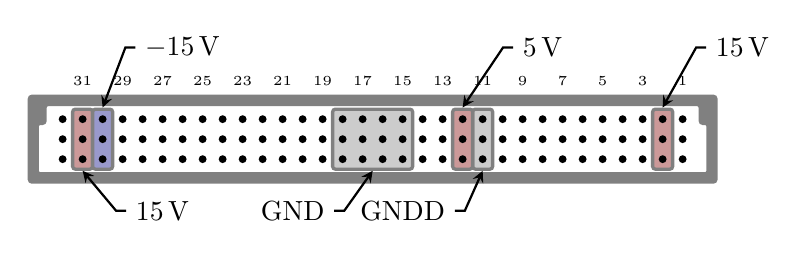
\begin{tikzpicture}[x=2.54mm, y=2.54mm,
        outline/.style = {%
            rectangle,%
            rounded corners=1,%
            very thick,%
            draw=black!50,%
            fill=black!50,%
            minimum height=10.9mm,%
            minimum width=87.2mm,%
            outer sep=0pt,%
        },%
        marker/.style = {%
            rectangle,%
            rounded corners=1,%
            very thick,%
            draw=black!50,%
        },%
        positive voltage/.style = {%
            fill=red!50!black!40,%
        },%
        negative voltage/.style = {%
            fill=blue!50!black!40,%
        },%
        ground/.style = {%
            fill=white!50!black!40,%
        },%
        pin/.style = {%
            fill=black,%
            circle,minimum size=1mm,%
            inner sep=0pt,%
        },%
        arrow/.style = {%
            thick,%
            ->,%
            >=stealth,%
        },%
        ]
        % Outer border
        \node[outline] (OUTER) at (15.5,1) {};
        % Inner border
        \draw[rounded corners=1, very thick, draw=black!50, fill=white] (OUTER.south west) ++ (1mm,1.05mm) -- ++(0,6.4mm) -- ++(1mm,0) -- ++ (0,2.4mm) -- ++(83.2mm,0) -- ++(0,-2.4mm) -- ++(1mm,0) -- ++(0,-6.4mm) -- cycle;
        % Marker
        \node[marker, positive voltage, minimum height=3*2.54mm, minimum width=1*2.54mm] (POSITIVE) at (30,1) {};
        \node[marker, positive voltage, minimum height=3*2.54mm, minimum width=1*2.54mm] (POSITIVE_OPTION) at (1,1) {};
        \node[marker, ground, minimum height=3*2.54mm, minimum width=4*2.54mm] (GND) at (15.5,1) {};
        \node[marker, ground, minimum height=3*2.54mm, minimum width=1*2.54mm] (GNDD) at (21,1) {};
        \node[marker, positive voltage, minimum height=3*2.54mm, minimum width=1*2.54mm] (5V) at (20,1) {};
        \node[marker, negative voltage, minimum height=3*2.54mm, minimum width=1*2.54mm] (NEGATIVE) at (2,1) {};
        % Pins
        \foreach \i in {0,...,31} {
            \foreach \j in {0,...,2} {
                \node[pin] at (\i,\j) {};
            }
        }
        \foreach \i in {1,3,...,32} {
            \node[above=3mm] at (32-\i,2) {\tiny \i};
        }
        % Labels
        \node[] (POSITIVE_LABEL) at ($(POSITIVE.north) + (4,3)$) {\SI{15}{\V}};
        \draw[arrow] (POSITIVE_LABEL.west) -- ++(-0.5,0) -- (POSITIVE.north);
        \node[] (5V_LABEL) at ($(5V.north) + (4,3)$) {\SI{5}{\V}};
        \draw[arrow] (5V_LABEL.west) -- ++(-0.5,0) -- (5V.north);
        \node[] (GND_LABEL) at ($(GND.south) + (-4,-2)$) {GND};
        \draw[arrow] (GND_LABEL.east) -- ++(0.5,0) -- (GND.south);
        \node[] (GNDD_LABEL) at ($(GNDD.south) + (-4,-2)$) {GNDD};
        \draw[arrow] (GNDD_LABEL.east) -- ++(0.5,0) -- (GNDD.south);
        \node[] (NEGATIVE_LABEL) at ($(NEGATIVE.north) + (4,3)$) {\SI{-15}{\V}};
        \draw[arrow] (NEGATIVE_LABEL.west) -- ++(-0.5,0) -- (NEGATIVE.north);
        \node[] (POSITIVE_OPTION_LABEL) at ($(POSITIVE_OPTION.south) + (4,-2)$) {\SI{15}{\V}};
        \draw[arrow] (POSITIVE_OPTION_LABEL.west) -- ++(-0.5,0) -- (POSITIVE_OPTION.south);
    \end{tikzpicture}
\end{document}
